\documentclass[tikz,border=5pt]{standalone}
\usepackage{amsmath}

\begin{document}
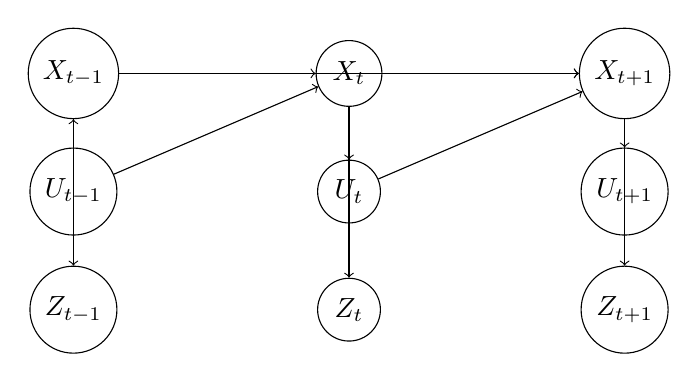
\begin{tikzpicture}[node distance=1.5cm, auto]
    % Time t-1
    \node (Xt_1) [draw, circle] {\( X_{t-1} \)};
    \node (Ut_1) [draw, circle, below of=Xt_1] {\( U_{t-1} \)};
    \node (Zt_1) [draw, circle, below of=Ut_1] {\( Z_{t-1} \)};

    % Time t
    \node (Xt) [draw, circle, right of=Xt_1, xshift=2cm] {\( X_t \)};
    \node (Ut) [draw, circle, below of=Xt] {\( U_t \)};
    \node (Zt) [draw, circle, below of=Ut] {\( Z_t \)};

    % Time t+1
    \node (Xt_1p) [draw, circle, right of=Xt, xshift=2cm] {\( X_{t+1} \)};
    \node (Ut_1p) [draw, circle, below of=Xt_1p] {\( U_{t+1} \)};
    \node (Zt_1p) [draw, circle, below of=Ut_1p] {\( Z_{t+1} \)};

    % Arrows
    \draw[->] (Ut_1) -- (Xt_1);
    \draw[->] (Xt_1) -- (Zt_1);
    \draw[->] (Xt_1) -- (Xt);
    \draw[->] (Ut_1) -- (Xt);
    \draw[->] (Xt) -- (Ut);
    \draw[->] (Xt) -- (Zt);
    \draw[->] (Xt_1) -- (Xt_1p);
    \draw[->] (Ut) -- (Xt_1p);
    \draw[->] (Xt) -- (Xt_1p);
    \draw[->] (Xt_1p) -- (Ut_1p);
    \draw[->] (Xt_1p) -- (Zt_1p);
\end{tikzpicture}
\end{document}
